\documentclass[10pt,a4paper]{article}

% Layout and typography
\usepackage[a4paper,margin=2.1cm]{geometry}
\usepackage[T1]{fontenc}
\usepackage{lmodern}
\usepackage[english]{babel}
\usepackage{microtype}
\usepackage{setspace}
\usepackage{graphicx}
\usepackage{float} % Provides [H] placement for figures

% Mathematics, tables, and links
\usepackage{amsmath,amssymb}
\usepackage{booktabs,tabularx}
\usepackage{xcolor}
\usepackage{hyperref}

\definecolor{navy}{RGB}{24,54,96}
\hypersetup{
    colorlinks=true,
    linkcolor=navy,
    citecolor=navy,
    urlcolor=navy
}
\setlength{\parskip}{3pt}
\setlength{\parindent}{1em}
\setlength{\textfloatsep}{10pt}
\setlength{\intextsep}{8pt}
\setlength{\abovecaptionskip}{4pt}
\setlength{\belowcaptionskip}{2pt}

\title{Modeling Caribbean Coral Reef Hysteresis \& Parrotfish Dynamics}
\author{Gent Maksutaj\\
\small MA 311, Colby College}
\date{}

\begin{document}
\maketitle

\begin{abstract}
Caribbean coral reefs have shifted from coral-dominated communities to degraded reefs covered by macroalgae. Following the mass mortality of the sea urchin \textit{Diadema antillarum} in 1983--1984, parrotfishes became the main grazers limiting algal growth. Using the model of Blackwood, Hastings, and Mumby (2012), we study how fishing and coral-dependent parrotfish carrying capacity affect reef stability. We compare food limitation, where coral reduces algal foraging area, with habitat limitation, where coral provides shelter. The analysis shows that habitat-limited reefs tolerate less fishing and may not recover naturally after collapse. Simulations further show that moderate fishing can permit slow recovery under food limitation but cause collapse under habitat limitation.
\end{abstract}

\section{Introduction}

Coral reefs provide coastal protection, fisheries habitat, and biodiversity, but Caribbean reefs have undergone substantial degradation \cite{hughes1994,jackson2014}. Historically, parrotfishes and the long-spined sea urchin \textit{Diadema antillarum} controlled macroalgae. A waterborne pathogen killed more than 90\% of these urchins across the Caribbean in 1983--1984, leaving parrotfishes as the dominant grazers \cite{hughes1994,bellwood2004,mumby2007}.

Some reefs exhibit \textit{hysteresis}: after a shift from coral to macroalgal dominance, simply reducing fishing may not restore the original state. Feedbacks between coral, habitat, and grazing can keep a reef degraded even after the pressure that caused its collapse is removed \cite{mumby2007,blackwood2012}.

Fishing regulations vary across the Caribbean. A regional review found that, among 37 responding jurisdictions, 12 had complete parrotfish-harvest bans, 12 had partial restrictions, and 13 had no species-specific regulations \cite{harmstuohy2021}. Understanding the fishing levels reefs can tolerate is therefore important for management.

Mumby, Hastings, and Edwards \cite{mumby2007} modeled coral, macroalgae, and turf under constant grazing. Blackwood, Hastings, and Mumby \cite{blackwood2012} extended this model by allowing parrotfish abundance to respond to fishing and coral cover. We use their framework to compare food- and habitat-limited carrying capacities, identify fishing thresholds, and examine how fishing and ecological parameters affect reef recovery. Section 2 presents the model, Section 3 analyzes its equilibria, Section 4 reports simulations and sensitivity results, and Section 5 discusses management implications.

\section{Mathematical Model}

\subsection{State Variables and Equations}

We represent a reef patch using three benthic cover fractions: macroalgae $M(t)$, live coral $C(t)$, and short algal turf $T(t)$. They satisfy
\begin{equation}
    M+C+T=1,\qquad M,C,T\geq 0,
    \label{eq:conservation}
\end{equation}
so $T=1-M-C$. Parrotfish abundance is represented by $P(t)\in[0,1]$, scaled to maximum unfished carrying capacity.

Following Blackwood et al. \cite{blackwood2012}, the system is
\begin{align}
    \frac{dM}{dt} &= aMC-\frac{PM}{M+T}+\gamma MT, \label{eq:dM}\\
    \frac{dC}{dt} &= rTC-dC-aMC, \label{eq:dC}\\
    \frac{dP}{dt} &= sP\left(1-\frac{P}{K(C)}\right)-fP, \label{eq:dP}
\end{align}
where $T=1-M-C$. Macroalgae spreads over coral and turf, but grazing converts macroalgae to turf. Coral recruits onto turf and is lost through natural mortality and macroalgal overgrowth. Parrotfish grow logistically toward carrying capacity $K(C)$ and experience fishing mortality $f$.

\begin{table}[htbp]
\centering
\small
\caption{Model parameters and baseline values \cite{mumby2007,blackwood2012}.}
\label{tab:parameters}
\begin{tabularx}{\textwidth}{@{}l c c X@{}}
\toprule
Parameter & Symbol & Value & Description\\
\midrule
Coral overgrowth & $a$ & $0.10$ & Macroalgal overgrowth of coral\\
Macroalgal spread & $\gamma$ & $0.80$ & Spread across turf\\
Coral recruitment & $r$ & $1.00$ & Coral growth on turf\\
Coral mortality & $d$ & $0.44$ & Natural coral loss\\
Parrotfish growth & $s$ & $0.49$ & Intrinsic population growth\\
Food limitation & $z$ & $0.50$ & Effect of coral on foraging area\\
Fishing mortality & $f$ & $0$--$0.50$ & Parrotfish harvesting\\
\bottomrule
\end{tabularx}
\end{table}
All rates are in $\mathrm{yr}^{-1}$; $z$ is dimensionless.

\subsection{Carrying Capacity and Assumptions}

We compare two formulations from Blackwood et al. \cite{blackwood2012}:
\begin{align}
    K_{\mathrm{food}}(C)&=1-zC, \label{eq:Kfood}\\
    K_{\mathrm{hab}}(C)&=C. \label{eq:Khab}
\end{align}
In the food-limited model, coral reduces the area available for algal foraging. In the habitat-limited model, coral structure provides shelter from predators. Thus, coral loss also reduces parrotfish carrying capacity, weakening grazing and promoting further coral loss.

The model treats the reef as spatially uniform and fishing pressure as constant. It also combines parrotfish species and size classes into one population. These assumptions simplify the analysis but omit spatial variation, fisher responses, and species-specific ecology.

\section{Equilibrium and Stability Analysis}

\subsection{Equilibria and Fishing Thresholds}

Equilibria are found by setting the derivatives in Equations \eqref{eq:dM}--\eqref{eq:dP} to zero. When $f\geq s$, parrotfish become extinct. For $f<s$ and positive carrying capacity, the parrotfish equilibrium is
\begin{equation}
    P^*(C)=K(C)\left(1-\frac{f}{s}\right).
    \label{eq:Pstar}
\end{equation}

The coral-dominated equilibrium has no macroalgae. From the coral equation,
\begin{equation}
    C^*=1-\frac{d}{r}=0.56,\qquad T^*=\frac{d}{r}=0.44.
    \label{eq:coraleq}
\end{equation}
Its stability depends on whether grazing is strong enough to prevent macroalgae from invading. The critical grazing level is
\begin{equation}
    P_{\mathrm{crit}}=(1-C^*)[aC^*+\gamma(1-C^*)]=0.17952.
    \label{eq:Pcrit}
\end{equation}
Setting $P^*(C^*)=P_{\mathrm{crit}}$ gives the critical fishing rate:
\begin{equation}
    f_{\mathrm{crit}}=s\left(1-\frac{P_{\mathrm{crit}}}{K(C^*)}\right).
    \label{eq:fcrit}
\end{equation}
The resulting thresholds are
\begin{equation}
    f_{\mathrm{crit}}^{\mathrm{food}}\approx0.3678,\qquad
    f_{\mathrm{crit}}^{\mathrm{hab}}\approx0.3329
    \quad \mathrm{yr}^{-1}.
\end{equation}
Thus, habitat-limited reefs lose stability at a lower fishing rate.

\subsection{Bistability and Hysteresis}

The degraded macroalgal equilibrium is $E_{\mathrm{alg}}=(1,0,0)$. Under food limitation, parrotfish can return when fishing is below their growth rate, $s=0.49$. The lower boundary of the hysteresis interval is approximately $f=0.2976$. Between this value and the coral-collapse threshold, the long-term outcome depends on the initial reef state. Below the lower boundary, any positive initial coral cover can recover.

Under habitat limitation, $K(C)$ approaches zero as coral disappears. The degraded state therefore remains locally stable at every non-negative fishing rate. Once coral falls below the unstable boundary separating recovery from collapse, stopping fishing alone cannot restore the reef. This is the key difference between the two carrying-capacity assumptions.

\begin{table}[htbp]
\centering
\small
\caption{Equilibrium stability and hysteresis under the baseline parameters.}
\label{tab:equilibria}
\begin{tabularx}{\textwidth}{@{}l X X@{}}
\toprule
 & \textbf{Food-limited} & \textbf{Habitat-limited}\\
\midrule
Coral state & Stable for $f<0.3678$ & Stable for $f<0.3329$\\
Degraded state & Stable only when $f>0.49$ & Stable for all $f\geq0$\\
Hysteresis interval & $0.2976<f<0.3678$ & $0\leq f<0.3329$\\
\bottomrule
\end{tabularx}
\end{table}

\section{Numerical Simulations and Sensitivity}

\subsection{Simulation Setup}

We numerically solved Equations \eqref{eq:dM}--\eqref{eq:dP} using the fourth-order Runge--Kutta method (RK4) in Python with a time step of $\Delta t=0.02\,\mathrm{yr}$ over a $120$-year horizon. Both experiments started from a degraded reef state with low coral ($C_0=0.20$) and parrotfish ($P_0=0.05$), and macroalgae initialized at its corresponding equilibrium $M_0=(1-C_0)+(aC_0-P_0/(1-C_0))/\gamma=0.7469$:
\begin{equation}
    (M_0,C_0,P_0)=(0.7469,0.2,0.05),\qquad T_0=0.0531.
    \label{eq:IC}
\end{equation}
We conducted two separate simulation experiments across three fishing regimes: no fishing ($f=0\,\mathrm{yr}^{-1}$), intermediate fishing ($f=0.25\,\mathrm{yr}^{-1}$), and heavy fishing ($f=0.45\,\mathrm{yr}^{-1}$)—defining coral recovery time as the first time $C\ge 0.5$. The sole difference between the two experiments is how parrotfish carrying capacity $K(C)$ depends on coral cover:
\begin{enumerate}
    \item Food-limited experiment: Carrying capacity decreases linearly with coral cover as $K(C)=1-zC$, reflecting greater algal food availability on degraded reefs.
    \item Habitat-limited experiment: Carrying capacity scales directly with structural coral habitat as $K(C)=C$.
\end{enumerate}

\subsection{Food-Limited Case}

Under food limitation ($K(C)=1-zC$), algal abundance on the degraded reef initially supports strong parrotfish growth, enabling recovery when fishing stays below $f_{\mathrm{crit}}^{\mathrm{food}}=0.3678\,\mathrm{yr}^{-1}$:
\begin{itemize}
    \item No fishing ($f=0\,\mathrm{yr}^{-1}$): Grazing suppresses macroalgae and restores the coral-dominated equilibrium ($C=0.56$, $M=0$, $P=0.72$), reaching $C\ge 0.50$ in $19.1\,\mathrm{yr}$.
    \item Intermediate fishing ($f=0.25\,\mathrm{yr}^{-1}$): Because $f<f_{\mathrm{crit}}^{\mathrm{food}}$, the reef still reaches the coral-dominated equilibrium ($C=0.56$, $M=0$, $P=0.353$), but reduced grazer density delays recovery ($C\ge 0.50$) to $65.9\,\mathrm{yr}$.
    \item Heavy fishing ($f=0.45\,\mathrm{yr}^{-1}$): Fishing exceeds $f_{\mathrm{crit}}^{\mathrm{food}}$ and depletes parrotfish ($P=0.081$), causing coral collapse ($C=0$) and macroalgal dominance ($M=0.899$).
\end{itemize}

\begin{figure}[H]
\centering
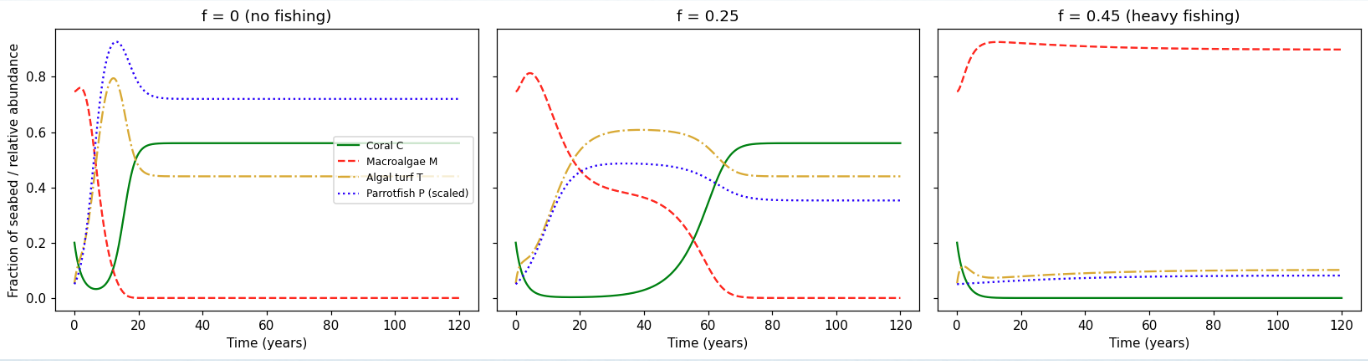
\includegraphics[width=0.9\textwidth]{food_limited.png}
\caption{Time series of coral ($C$), macroalgae ($M$), and parrotfish ($P$) over 120 years under the food-limited model ($K(C)=1-zC$) for fishing rates $f=0$, $0.25$, and $0.45\,\mathrm{yr}^{-1}$.}
\label{fig:food_limited}
\end{figure}

\subsection{Habitat-Limited Case}

Under habitat limitation ($K(C)=C$), we set $f=0\,\mathrm{yr}^{-1}$ (the most favorable fishing condition) and test two initial condition sets to evaluate hysteresis:
\begin{itemize}
    \item Low initial macroalgae ($M_0=0.1$): Available coral shelter sustains enough grazing to suppress macroalgae, allowing convergence to the coral-dominated equilibrium ($C=0.56$, $M=0$, $P=0.56$).
    \item High initial macroalgae ($M_0=0.5$): Macroalgal overgrowth outpaces habitat-limited grazing, driving coral collapse ($C=0$, $M=0.987$, $P=0.01$).
\end{itemize}
This divergence confirms hysteresis under habitat limitation: even without fishing, the reef's long-term state depends on its initial macroalgal cover.

\begin{figure}[H]
\centering
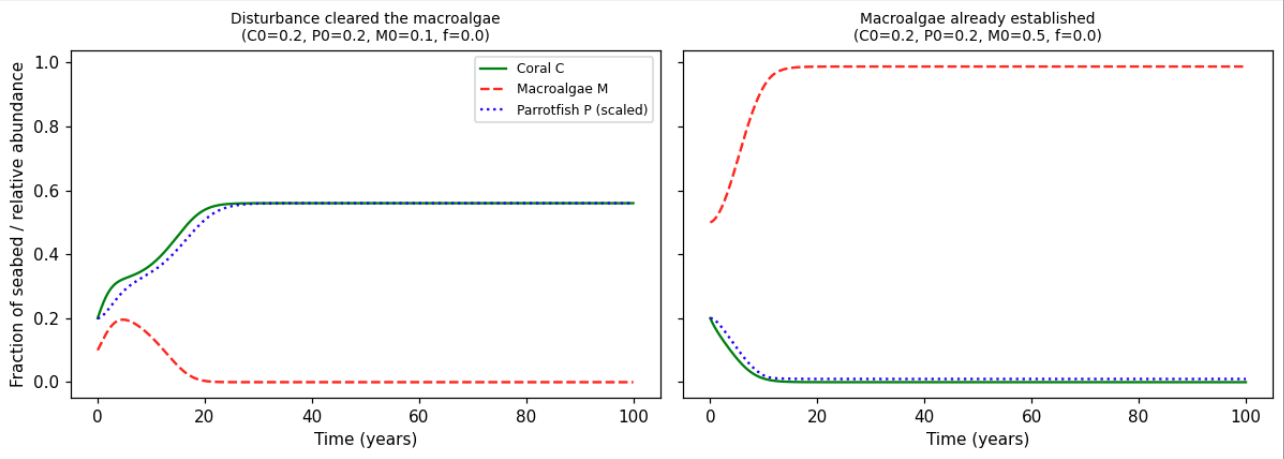
\includegraphics[width=0.9\textwidth]{habitat_limited.png}
\caption{Time series of coral ($C$), macroalgae ($M$), and parrotfish ($P$) over 120 years under the habitat-limited model ($K(C)=C$) for initial macroalgal covers $M_0=0.1$ and $M_0=0.5$.}
\label{fig:habitat_limited}
\end{figure}

\subsection{Parameter Sensitivity}

We varied parrotfish growth ($s$), macroalgal spread ($\gamma$), and food limitation ($z$) individually to examine their effects on the critical fishing thresholds.

\begin{table}[htbp]
\centering
\small
\caption{Critical fishing thresholds under parameter changes.}
\label{tab:sensitivity}
\begin{tabularx}{\textwidth}{@{}l c c c X@{}}
\toprule
Parameter & Value & $f_{\mathrm{crit}}^{\mathrm{food}}$ & $f_{\mathrm{crit}}^{\mathrm{hab}}$ & Main effect\\
\midrule
Baseline & --- & 0.3678 & 0.3329 & Reference case\\
$s$ & 0.40 & 0.3003 & 0.2718 & Slower parrotfish growth lowers both thresholds\\
$s$ & 0.50 & 0.3753 & 0.3397 & Faster growth raises both thresholds\\
$\gamma$ & 0.60 & 0.3942 & 0.3668 & Slower algal spread raises thresholds\\
$\gamma$ & 1.00 & 0.3415 & 0.2990 & Faster algal spread lowers thresholds\\
$z$ & 0.25 & 0.3877 & 0.3329 & Weaker food limitation raises the food threshold\\
$z$ & 0.75 & 0.3383 & 0.3329 & Stronger food limitation lowers the food threshold\\
\bottomrule
\end{tabularx}
\end{table}

The results show that reefs tolerate less fishing when parrotfish grow more slowly or macroalgae spreads faster. Stronger food limitation also makes the food-limited threshold approach the habitat-limited threshold. Overall, both grazer population growth and algal spread influence reef resilience.

\section{Discussion and Conclusion}

The carrying-capacity mechanism strongly affects reef resilience. Habitat-limited reefs tolerate less fishing than food-limited reefs, and their degraded state can persist even when fishing stops. The simulations illustrate this difference: at intermediate fishing, food-limited reefs recover slowly while habitat-limited reefs collapse.

These results have practical implications for Caribbean management. Fishing restrictions are important, but may not be enough once a habitat-limited reef has lost most of its coral structure. Such reefs may also require active restoration, such as coral outplanting or macroalgal removal. Preventing reefs from crossing collapse thresholds is therefore especially important. Reducing nutrient runoff and protecting parrotfish populations can help maintain the grazing and habitat conditions needed for recovery.

\section*{Code Availability}
Python scripts for the RK4 simulations and the source code of this paper are available at \href{https://github.com/gentmaks/MA311-Final-Project}{the project GitHub page}.

\begin{thebibliography}{9}
\small

\bibitem{bellwood2004}
Bellwood, D. R., Hughes, T. P., Folke, C., \& Nystr{\"o}m, M. (2004).
Confronting the coral reef crisis. \textit{Nature}, 429(6994), 827--833.

\bibitem{blackwood2012}
Blackwood, J. C., Hastings, A., \& Mumby, P. J. (2012).
The effect of fishing on hysteresis in Caribbean coral reefs.
\textit{Theoretical Ecology}, 5(1), 105--114.

\bibitem{harmstuohy2021}
Harms-Tuohy, C. A. (2021).
\textit{Parrotfishes in the Caribbean: A regional review with recommendations for management}.
FAO Fisheries and Aquaculture Circular No. 1240. Rome: FAO.

\bibitem{hughes1994}
Hughes, T. P. (1994).
Catastrophes, phase shifts, and large-scale degradation of a Caribbean coral reef.
\textit{Science}, 265(5178), 1547--1551.

\bibitem{jackson2014}
Jackson, J. B. C., Donovan, M. K., Cramer, K. L., \& Lam, V. V. (Eds.). (2014).
\textit{Status and trends of Caribbean coral reefs: 1970--2012}.
Gland, Switzerland: Global Coral Reef Monitoring Network, IUCN.

\bibitem{mumby2007}
Mumby, P. J., Hastings, A., \& Edwards, H. J. (2007).
Thresholds and the resilience of Caribbean coral reefs.
\textit{Nature}, 450(7166), 98--101.

\end{thebibliography}
\end{document}
